% In your .tex file

\documentclass{article} % For LaTeX2e
\usepackage{nips15submit_e,times}
\usepackage{xparse}
\usepackage{subcaption}

\usepackage{hyperref}
\usepackage{url}
\usepackage[toc,page]{appendix}
% \usepackage{icml2015}

%citation
\usepackage[backend=bibtex]{biblatex}
\bibliography{main}
%

% tikz and associated macros
\usepackage{tikz}
\usepackage{tikz-cd}

\usepackage{pgfplots}
\newcommand\sep{1.9cm}
\newcommand\height{0.9cm}
\usetikzlibrary{decorations.pathmorphing, backgrounds}
\tikzset{snake it/.style={decorate, decoration=snake}}
%
%

% math
\usepackage{amsthm}
\usepackage{amsmath}
\usepackage{amssymb}
\usepackage{mathabx}

\newcommand{\BlackBox}{\rule{1.5ex}{1.5ex}}  % end of proof
\newtheorem{example}{Example}
\newtheorem{theorem}{Theorem}
\newtheorem{lemma}[theorem]{Lemma}
\newtheorem{proposition}[theorem]{Proposition}
\newtheorem{remark}[theorem]{Remark}
\newtheorem{corollary}[theorem]{Corollary}
\newtheorem{definition}[theorem]{Definition}
\newtheorem{conjecture}[theorem]{Conjecture}
\newtheorem{axiom}[theorem]{Axiom}

\numberwithin{equation}{subsection}
\numberwithin{theorem}{subsection}

\DeclareSymbolFont{cmlargesymbols}{OMX}{cmex}{m}{n}
\let\sumop\relax
\DeclareMathSymbol{\sumop}{\mathop}{cmlargesymbols}{"50}


\def\reals{{\mathbb R}}
\def\torus{{\mathbb T}}
\def\integers{{\mathbb Z}}
\def\rationals{{\mathbb Q}}
\def\expect{\mathop{{\mathbb{E}}}}
\def\tens{\mathop{{\bigotimes}}}
\def\naturals{{\mathbb N}}
\def\complex{{\mathbb C}\/}
\def\distance{\operatorname{distance}\,}
\def\support{\operatorname{support}\,}
\def\dist{\operatorname{dist}\,}
\def\Span{\operatorname{span}\,}
\def\degree{\operatorname{degree}\,}
\def\kernel{\operatorname{kernel}\,}
\def\dim{\operatorname{dim}\,}
\def\codim{\operatorname{codim}}
\def\trace{\operatorname{trace\,}}
\def\dimension{\operatorname{dimension}\,}
\def\codimension{\operatorname{codimension}\,}
\def\kernel{\operatorname{Ker}}
\def\Re{\operatorname{Re\,} }
\def\Im{\operatorname{Im\,} }
\def\eps{\varepsilon}
\def\lt{L^2}
\def\bull{$\bullet$\ }
\def\det{\operatorname{det}}
\def\Det{\operatorname{Det}}
\def\diameter{\operatorname{diameter}}
\def\symdif{\,\Delta\,}
\newcommand{\norm}[1]{ \|  #1 \|}
\newcommand{\set}[1]{ \left\{ #1 \right\} }
\def\suchthat{\mathrel{}\middle|\mathrel{}}
\def\one{{\mathbf 1}}
\def\cl{\text{cl}}

\def\newbull{\medskip\noindent $\bullet$\ }
\def\nobull{\noindent$\bullet$\ }
\def\defeq{\stackrel{\text{def}}{=}}

\newtheoremstyle{named}{}{}{\itshape}{}{\bfseries}{.}{.5em}{\thmnote{#3's }#1}
\theoremstyle{named}
\newtheorem*{namedtheorem}{Theorem}



\def\scriptf{{\mathcal F}}
\def\scriptq{{\mathcal Q}}
\def\scriptg{{\mathcal G}}
\def\scriptm{{\mathcal M}}
\def\scriptb{{\mathcal B}}
\def\scriptc{{\mathcal C}}
\def\scriptt{{\mathcal T}}
\def\scripti{{\mathcal I}}
\def\scripte{{\mathcal E}}
\def\scriptv{{\mathcal V}}
\def\scriptw{{\mathcal W}}
\def\scriptu{{\mathcal U}}
\def\scriptS{{\mathcal S}}
\def\scripta{{\mathcal A}}
\def\scriptr{{\mathcal R}}
\def\scripto{{\mathcal O}}
\def\scripth{{\mathcal H}}
\def\scriptd{{\mathcal D}}
\def\scriptl{{\mathcal L}}
\def\scriptn{{\mathcal N}}
\def\scriptp{{\mathcal P}}
\def\scriptk{{\mathcal K}}
\def\scriptP{{\mathcal P}}
\def\scriptj{{\mathcal J}}
\def\scriptz{{\mathcal Z}}
\def\scripts{{\mathcal S}}
\def\scriptx{{\mathcal X}}
\def\scripty{{\mathcal Y}}
\def\frakv{{\mathfrak V}}
\def\frakG{{\mathfrak G}}
\def\frakB{{\mathfrak B}}
\def\frakC{{\mathfrak C}}



%\todo[inline]v %NOTES. To remove for camera ready version.
\usepackage{todonotes}
\usepackage{regexpatch}
%end to notes

\title{Backpropagation-Free Parallel Deep Reinforcement Learning}

\author{
William H.~Guss \\
Machine Learning at Berkeley\\
\texttt{wguss@ml.berkeley.edu} \\
\And
Phillip Kuznetsov \\
Machine Learning at Berkeley \\
Berkeley CA, 94720 \\
\texttt{mlyzhong@berkeley.edu} \\
\And
Noah Golmant\\
Machine Learning at Berkeley\\
Berkeley CA, 94720 \\
\texttt{noah.golmant@berkeley.edu}
\And
Max Johansen \\
Machine Learning at Berkeley \\
Berkeley CA, 94720 \\
\texttt{max@ml.berkeley.edu}
}



\nipsfinalcopy % Uncomment for camera-ready version

\begin{document}


\maketitle

\begin{abstract}
    In this paper we conjecture that an agent, envirionment pair $(\mu, E)$ trained using DDPG with an actor network $\mu$ and critic network $Q^{\mu}$ can be decomposed into a number of sub-agent, sub-environment pairs  $(\mu^n, E^n)$ ranging over every neuron in $\mu$; that is, we show empirically that treating each neuron $n$ as an agent $\mu^n: \mathbb{R}^n \to \mathbb{R}$ of its inputs and optimizing a value function $Q^{\mu^n}$ with respect to the weights of $\mu^n$ is dual to optimizing $Q^\mu$ with respect to the weights of $\mu$. Finally we propose a learning rule which simultaneously optimizes each $\mu^n$ without error backpropogation achieving state of the art performance and speed across a variety of OpenAI Gym environments.
\end{abstract}
% \listoftodos

\section{Introduction}
Recent techniques in deep reinforcement learning attempt to learn two deep neural networks: one to approximate a value function and one to learn a deterministic policy that maximizes this value function according to the action the agent performs.  

Other work has attempted to address the issue of decoupling connections between layers in the network using decoupled neural interfaces \cite{DBLP:journals/corr/JaderbergCOVGK16}. Synthetic gradient modules model the error gradient using only local information, allowing immediate feedback that is later corrected when the backpropogated error is finally computed. This method has had significant successes in both feedforward and recurrent architectures.

Both of these techniques still rely on biologically implausible backpropagation mechanisms to learn the parameters of the networks. We attempt to address these issues by decomposing the agent and learning rules at the local neuron level.

\section{Agent-Environment Value Decomposition}

In this section we will develop a theoretical basis for decomposing the agent and its environment into local agents which take in prior neuron activations as state and output activations as the neuron's own actions. We will then show that under some mild conditions, these agents act in environments which are so simple that it suffices to estimate the policy gradient using a linear approximation. These results lead to a new decentralized, local, and asynchronous learning paradigm for deep reinforcement learning without the use of deep error-backpropagation.

\subsection{Background}
Recall the standard reinforcement learning setup. We say $E$ is an \emph{environment} if $E \defeq (\scripts, \scripta, \scriptr, T, r)$ where $T$ describes transition probability measure $T\left(s_{t+1}\suchthat s_t, a_t\right)$ and $r: \scripts \times \scripta \to \scriptr$ is a reward function. Furthermore $\scripts$, $\scripta$, $\scriptr$ are the \emph{state space, action space, and reward space} respectively. We restrict $\scriptr$ to a compact subset of $\mathbb{R}$ and action space and state space to finite dimensional real vector spaces. As in DDPG \cite{DBLP:journals/corr/LillicrapHPHETS15} we assume that the environment $E$ is \emph{fully observed}; that is, at any time step the state $s_t$ is fully described by the observation presented, $x_t$, and not by the history $(x_1, a_1, \dots, a_{t-1}).$

We define the policy for an agent to be $\mu: \scriptp(\scripta) \times \scripts \to [0,1]$. We will deal only with \emph{deterministic} policies where for every $s_t$ there is unique $a_t$ so that $\mu\left(\set{a_t} \suchthat s = s_t\right) = 1$ and the measure is $0$ otherwise. Thus we define a \emph{deterministic agent} by a policy function $\mu: \scripts \to \scripta$. Additionally we denote the state-space trajectories of $\mu $ by
\begin{equation}
 	\Gamma_\mu(\scripts) = \set{((s_1, a_1), (s_2, a_2) \dots)\suchthat s_1 \sim T(s_0), s_{t+1} \sim T\left(s \suchthat s_t, \mu(s_t)\right)}.
 \end{equation}

For a policy $\mu$  the action-value function is the expected future reward under $\mu$ by performing $a_t$ at state $s_t$. A temporally local definition thereof can be obtained using the Bellman equation
\begin{equation}
    Q^{\mu}(s_t, a_t) = \expect_{s_{t+1} \sim E}\left[r(s_{t}, a_t) + \gamma Q^{\mu}(s_{t+1}, \mu(s_{t+1}))\right]
\end{equation}
with $\gamma \in (0,1)$ a discount factor, and the second expectation removed because $\mu$ is deterministic.

Among a variety of methods, the deep reinforcement learning approach to solving environments (MDPs) has predominately been separated into deterministic policy gradient methods and direct, optimal Q-Learning methods. In deterministic policy gradient (DPG) methods, we define an actor $\mu: \scripts \to \scripta$ and a critic $Q^\mu: \scripts \times \scripta \to \mathbb{R}$ and optimize $Q^\mu(s_t, \mu(s_t | \theta^{\mu}))$ with respect to the paramers $\theta^\mu$ of $\mu.$ Deep determinsiitc policy gradient (DDPG) learning directly learns to approximate $Q_a$ by creating two different deep neural networks for the actor and the critic and then back-propagating the $Q$ gradient from the critic to the actor. Specifically, DDPG maximizes $Q^\mu(s_t, \mu(s_t | \theta^{\mu}))$ with respect to the paramers $\theta^\mu$ of $\mu.$ This method is provably the true policy gradient of $\mu$ if $Q^\mu$ is known. In order to decompose the action-value function we will make heavy use of this methodology at a scale local to each neuron.

\subsection{Towards Neurocomputational Decomposition of $Q^\mu$}

In order to decompose the $Q^\mu$ algorithm we will abstractly define a neurocomputational agent in terms of an operator on voltages with no restrictions on the topology of the network, and then relate the action-value function of the whole agent to those which are defined for each individual neuron in the network.

\begin{definition}

If $\scriptv$ is an $N$-dimensional vector space then a \textbf{neurocomputational agent} is a tuple $\scriptn = (\mu, \epsilon, \delta, K, \Theta, \sigma, D)$ such that:
\begin{itemize}
    \item $\epsilon : \scripts  \to \scriptv$ encodes the state into the voltages. Realistically, only a subset of all neurons are input neurons, denoted as $N_I \subset \scriptv$, so $\epsilon(s_t) = \pi_{N_I}(\epsilon(s_t))$, where  $\pi_K(x)$ is the cannonical projection of $x$ on dimension(s) $K$,
    \item $\delta: \scriptv \to \scripta$ decodes the voltages of the \emph{output neurons } $N_O \subset V$ into an action, so that $\delta(v_t) = \delta(\pi_{N_O}(v_t))$.
    \item $K: \scriptv \to \scriptv$ is the linear voltage graph transition function of the graph representing the topolopy of $\scriptn$, parameterized by $\theta$.
    \item $\Theta: \scriptv \to \scriptv$ is a nonlinear inhibition function.
    \item $\sigma: \scriptv \to \scriptv$ is the elementwise application of some activation function to the voltage vector.
    \item $D: \scriptv \times \scriptv \to \scriptv$ is called voltage dynamic of $\scriptn$ such that
    \begin{equation}
        \begin{aligned}
         v_{t+1} \defeq D(v_t,v_{in}) \defeq \sigma\left(\Theta K[v_t]\right) + v_{in}
        \end{aligned}
    \end{equation}
    where $v_t$ is the internal voltage vector of $\scriptn$ at time $t$ and $v_{in}$ is an input voltage to the network. We will occasionally abuse notation an say that $D(v_t) = D(v_t, 0)$ when $v_{in}$ is 0.
    \item $\mu: \scripts \to \scripta$ is the deterministic policy for $\scriptn$ such that
    \begin{equation}
    	\begin{aligned}
        \mu(s_t) &= \delta(D(v_t, \epsilon(s_t))
    	\end{aligned}
    \end{equation}
\end{itemize}


\end{definition}


This definition encompasses any DQN or DDPG network with either reccurent or feedforward layers. In this paper we will mainly discuss standard feed forward neural networks, in which case $\Theta$ is not defined and the neural dynamics are repeatedly applied until an output of $N_O$ is produced.


\begin{definition}\label{def:subenv}

 If $n$ is some neuron in $\scriptn$, we say $E^n = (\scripts, \scripta, \scriptr, T^n, r^n)$ is a deterministic \textbf{sub-environment} of $E$ with respect to $\scriptn$ if

\begin{itemize}
  \item The state space is $\scripts = \scriptv$;  that is, the environment that neuron $n$ observes is the voltages of all other neurons. Although this definition permits a fully connected graph for $\scriptn$, realistically, each neuron only sees the voltages of a subset of all neurons. In the case of standard feed forward networks, $n$ would observe only the activations of the previous layer.

  \item The action space is the set of voltages $\scripta = \reals$ which the neuron $n$ can output.
  \item The reward space $\scriptr$ is the same as that of the base environment $E$. Furthermore the subenvironment emitts the same same reward as does the base environment. If the agent $\mu$ of $\scriptn$ acts on a state $s_t$ and receives a reward $r_t$, then every sub-environment emits the same reward $r_t$. 
  \item The transition function $T : \scriptv \times \mathbb{R}  \to \scripts ^n$ is such that 
  \begin{equation}
    T^n(v_t, \alpha_t) = (I - \chi_{n,n}) D(v_t)) + e_n \alpha + \epsilon(s_t)
  \end{equation}
  where $e_n$ is the $n^{th}$ unit basis vector, $I$ is the identity, and $\chi_{n,n} =1$ if $n = n$ and $0$ otherwise. Intuitively, the transition in $E^n$ is the normal\footnote{Since the state space of $E^n$ is only
  $\scriptv$, $s_t$ is a hidden variable of the markov decision process, and $T$ should be a function on $\scriptv \times \scripts \times \mathbb{R}$, but this is ommitted for simplicity.} neural dynamics on $\scriptn$ except for at the neuron $n$, itself; in $E^n$ we set the voltage of $n$ in $v_{t+1}$ to be the voltage chosen, $\alpha_t$, plus the newly encoded voltage $\epsilon(s_t)$.
\end{itemize}
 Lastly an agent  $\mu^n: \scriptv \to \mathbb{R}$  is called \textbf{neuromorphically local} to $\scriptn$ if $\mu^n: v_t \mapsto \langle D(v_t), e_n \rangle$; that is, $\mu^n$ acts according to the normal dynamics.

\end{definition}

With the basic definitions given, we will now show performing reinforcement learning on $\scriptn$ can be decomposed into the dual problem of perfoming reinforcement learning on agents and environments of type given in Definition \ref{def:subenv}.

\begin{theorem}[Neurocomputational Decompostion]\label{thm:ncomp}
  Let $E$ be an environment and $\scriptn$ be a neurocomputational agent. Then there exists a set of agent environment pairs $\mathfrak{D}_\scriptn \defeq \{(E^n, \mu^n)\}_{n\in \scriptn}$ such that for every $n \in \scriptn$, the following diagram commutes
\begin{equation}\label{eq:sub_env_com}
          \begin{tikzcd} %THe diagram for Q function decomposition.
%-------------------------------------------------------------------------------------%
        \scriptv  \times \scripts \arrow{r}{\mu\circ\pi_2}
             \arrow{d}
               {\pi_1  \times\epsilon \circ \pi_2}  &[+25pt]  \scripta    \\
%-------------------------------------------------------------------------------------%%
          \overbrace{\scriptv \times \scriptv}^{(v_{t},\epsilon(s_t))}
                      \arrow{r}{D}
                                  \arrow[pos = 0.7]{rd}[swap]{\mu^n\circ\pi_1 + \pi_n \circ \pi_2}
                      & \overbrace{\scriptv}^{v_{t+1}}
                                            \arrow[two heads, pos=0.8]
                                              {d}
                                              {\pi_n}
                                            \arrow{u}{\delta} \\
%%%%%%%%%%%%%%%%%%%%%%%%%%%%%%%%%%%%%%%%%%%%%%%%%%%%%%%%%%%%%%%%%%%%%%%%%%%%%%%%%%%%%%%
  &\reals
         \end{tikzcd}
    \end{equation}
\end{theorem}
\emph{Proof in Appendix}

Theorem \ref{thm:ncomp} gives a natural connection between the state space trajectories of $\mu$ and $\mu^n$ because in $\scriptn$, the voltage $v_t$ is a hidden variable which governs action of $\scriptn$ at any timestep and dually the state $s_t$ is a hidden variable of the Markov Decision Process formed by $E^n$ which governs the state given by $T^n$ at any timestep. 

Naturally, the following question arises: does DPG learning on $\scriptn$, specifically $\mu$ on $E$, commute with performing DPG learning on on every $(E^n, \mu^n) \in \mathfrak{D}_\scriptn$? Supposing that we have the true $Q^\mu$ function and $\mu$ is optimal with respect to $Q^\mu$, then it is intuitive, but not obvious, that every $\mu^n$ should behave optimally with respect to an $Q^{\mu^n}$ -- but will the reverse hold? To answer these questions we give the following result.
\begin{theorem}
    If $\scriptn$ is a nuerocomputational agent in $E$, then policy gradient for $\mu$ agrees with the simultaneous policy gradients of its decomposition; that is for every $(E^n, \mu^n) \in \mathfrak{D}_\scriptn$
    \begin{equation}\label{eq:ncompagrees}
        \nabla_{K^n} Q^{\mu^n}(v,\alpha)\Big|_{v=v_t,\alpha=\mu^n(v_t)} =\nabla_{K^n} Q^{\mu}(s,a)\Big|_{s=s_t,a=\mu(s_t)}
    \end{equation}
    for every time step $t$, where $K^n$ is the nth column of the linear voltage graph transition matrix, i.e. the weights of the connections from all neurons to neuron $n.$
\end{theorem}
\emph{Proof in Appendix}

Remarkably, the prevous theorem shows that optimizing every neuromorphically local agent $\mu^n$ with respect 
to a critic is exactly equivalent to optimizing the entire $\scriptn$ with respect to a global critic $Q^\mu$. 
Additionally optimization of the each $\mu^n$ does not require any backpropagation of $\nabla_a Q^{\mu^n}$ through the network since every $Q^{\mu^n}$ is diagramatically independent of eachother! As a result the neurocomputational decomposition $\mathfrak{D}_\scriptn$ of $\scriptn$ can be trained asynchronously and simultaneously.

\subsubsection{Simplicity of Sub-Environments}
An algorithm which learns $\scriptn$ by performing DPG learning on every $(E^n, \mu^n) \in \mathfrak{D}_\scriptn$ is only beneficial if each $Q^{\mu^n}$ can be approximated simply. For example if $Q^{\mu^n}$ are so complex that an approximation parameterized by $K$ requires more than $|K^n| \notin O(1)$ parameters, then standard error-backpropagation is sureley superior.

However the results established in \cite{DBLP:journals/corr/JaderbergCOVGK16} show that the approximation of the error backpropagated signal can be empircally linear in the activations. In the framework of DDPG, this intuitively says that the infintesmal effect of the weights $K^n$ on the dynamics and thereby the true $Q^\mu$ of a neurocomputational agent $\scriptn$ might be linear in the local neural neighborhood of $n$.

\section{Decentralized Deep Determinstic Policy Gradient Learning}
We use the preceding hypothesis as a motivation for the following local decomposition. We decompose the actor-critic dual networks of DDPG into a series of actor-critic pairs, where each actor neuron attempts to learn a local policy to maximize the value of its own critic. This critic is a linear regressor and its gradient agrees with the gradient of a global $Q$ network.

%!TEX root = main.tex
\section{Experimentation}
\subsection{Experiment 1: Learning Q functions on components of the Actor network.}

\textbf{Motivation:}
Our first batch of experiments aimed to establish empirically that the Q-functions of each layer, denoted $Q_1...Q_L$ are similar to the Q-function of the overall network, denoted $Q_{\mu}$. To that end, we extended the actor-critic methodology used in Lillicrap et al (2016) as follows. In addition to training $Q^\mu$, to estimate the Q functions of the actor network $\mu$, sub-critic networks $Q^n$ were initialized for each individual layer. We then compare the $Q$ values estimated by the subcritics to the $Q$ estimation provided by the main critic, $Q^\mu$. 


The inputs used in the calculation of the Q-functions for each layer follow the conceptual framework laid out in Section 2.2. The state and action parameters are therefore voltages represented by the outputs of $\epsilon : \scripts \to \scriptv$ and $\delta : \scriptv \to \scripta$ respectively, where the changes in voltage are described by a voltage transition function $K : \scriptv \to \scriptv$. 


To determine and compare the rate at which the subcritics and the main critic learn, the experiment was run in two phases. First, each of the subcritics and the main critic were trained using the standard DDPG algorithm on some actor $\mu$. In the second phase, a new actor $\mu'$ was initialized and its Q-function set to $Q_{\mu}$ as determined above in phase 1. The subcritics were trained, and the values of $Q_1\dots Q_{L}$ were plotted as training occurred.


After [number of iterations], each $Q^n(s,a)$  networks effectively learned the same cost function as $Q^{\mu}(s,a)$. Furthermore, the $Q$-value plots for each $Q^n$correlate directly with the  $Q^{\mu}$'s $Q$ plot. This confirms that we are able teach the $Q^n$ model on the level of subcomponents of $\mu$ supporting the argument that we can use $Q^n$ nets to approximate $Q^\mu$. We can now use each $Q^n$ to calculate the gradient of the specific neuron component that the $Q^n$ is critiquing. We proceed with this in Experiment 2.

\subsection{Experiment 2: Treating each neuron as its Actor-Critic network using linear approximators}

Now that we have established that the Critic networks for each of the individual neuron learns the same Q-function as does the entire agent, we now treat each neuron as its own actor. Each neuron changes the weights of its presynaptic neurons' connections, as parameters for its actor -- its voltage on the next timestep -- to optimize its learned approximated Q function. We use the linear approximation:

$$Q^{n}(v, a) \approx \theta_{n,v}^T v + \theta_{n,a}a = \theta_{n}^T (v, a)^T$$
$$\mu^{n}(v) = \sigma(K^n v)$$

GOT RID OF $\Theta$ in that it's not very necessary ...

IN CONCLUSION:

$$\theta_{n,v} \mathrel{+}= \frac{1}{N} \sum_i \eta_Q D_i v_i$$
$$\theta_{n,a} \mathrel{+}= \frac{1}{N} \sum_i \eta_Q D_i a_i$$
$$K^n \mathrel{+}= \frac{1}{N} \sum_i \eta_A \theta_{n,a} \sigma'(K^n v_i) v_i$$

where $D_i := (r_i + \gamma {\theta_n^T}' (v_{i+1}, a_{i+1})) - \theta_n (v_{i}, a_{i}) $

Intuitively, it should be the case that by treating each neuron in the neural network as its own Q-learner, the policy gradient of an individual agent should be the same as for the policy gradient entire agent, if each neuron sees the same reward $r_t$ as the entire agent. In other words, the optimal way of updating the entire connection matrix $K$ should be the optimal way for updating the weights connected to each neuron w.r.t. each neuron as its own Q-learner, given the same rewards.


\noindent 3. Plot the output of both $Q^\mu$ and $Qn$ using TENSORFLOW summaries.

From Experiment 1, we see that there is a correlation between the Q-gradient for neuron $n$, and the nth column of the gradient of the agent's Q function:

from strong to weak:
$$\nabla_{K^n} Q^{\mu^n}(v,a) = \nabla_{K^n} Q^{\mu}(s,a)$$
$$\nabla_{K^n} Q^{\mu^n}(v,a) \propto \nabla_{K^n} Q^{\mu}(s,a)$$
$$corr[\nabla_{K^n} Q^{\mu^n}(v,a), \nabla_{K^n} Q^{\mu}(s,a)] \approx EMPERICAL VALUE$$

although (assuming we get a weak experimental result), we propose that it is due to our neurons not being the ideal Q-learner (convergence issues, etc.).



\section{Results}

\subsection{Experiment 1}

We use the
\href{https://statistics.laerd.com/statistical-guides/pearson-correlation-coefficient-statistical-guide.php}{Pearson
correlation coefficient} to determine the similarity between the
derivatives of the global Q function critic and the local approximations
we use a-la DDPG.

The motivation of the paper states that we wish to approximate this
global Q using less expensive local Q approximator functions. We can
ignore the magnitude and actual values of the two functions as we only
wish to examine the updates, i.e.~derivatives of these functions. Thus,
we attempt to \textbf{find a positive correlation between
\(\frac{\partial Q_{global}}{\partial t}\) and
\(\frac{\partial Q_{local}}{\partial t}\).}

\href{https://statistics.laerd.com/statistical-guides/pearson-correlation-coefficient-statistical-guide.php}{According
to statistics.laerd.com}, this table can be used to roughly understand
the importance of correlations between two functions.

\begin{figure}[h]
\centering
\begin{subfigure}{.5\textwidth}
  \centering
  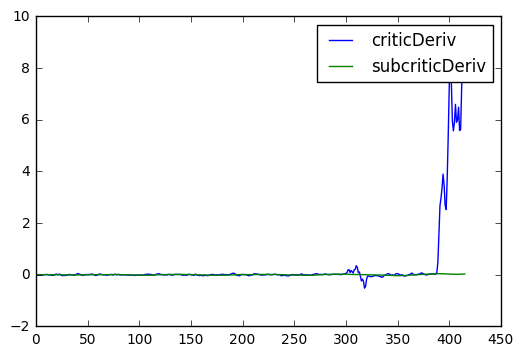
\includegraphics[width=.6\linewidth]{exp1_analysis_1_1.png}
  \caption{Critic and subcritic derivatives}
  \label{fig:sub1}
\end{subfigure}%
\begin{subfigure}{.5\textwidth}
  \centering
  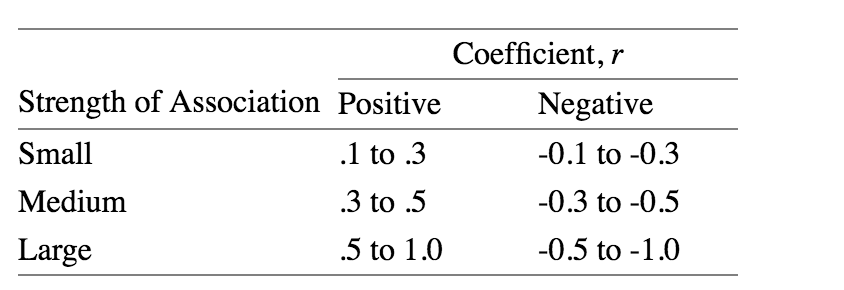
\includegraphics[width=.6\linewidth]{pearson_table.png}
  \caption{Pearson interpretation}
  \label{fig:sub2}
\end{subfigure}
\caption{Analysis figures}
\label{fig:test}
\end{figure}

In the mountain car experiment, we find a Pearson r-value of
0.389. Thus, we can infer that there is a ``weak
correlation'' between the derivatives of the global and local function.

These numbers are not necessarily significant without smoothing. As the
local approximations are inherently stochastic methods, we must apply
some smoothing techniques to obtain reasonable results.

\section{Conclusion}
The results of experiments 1 and 2 show that local learning rules are plausible. We were able to teach a network to perform a simple task in OpenAI gym using a small network structure. Furthermore, we should that we could employ local \emph{linear} learning rules to reach this end. This is shown in our results of experiment 2. 
\subsection{Future Work}
We want to scale our results to include truly deep neural network architectures. We show promising results using multi-layer networks, however we quickly fall victim to issues from high variance in large networks.

There are a number of techniques deep learning practitioners use to limit variance in standard deep learning architectures. 

One technique we're curious about is probabilistically fixing a subset of the neurons, while allowing the remaining neurons to \emph{explore}. This technique is very similar to the dropout used in deep learning research. We believe this will also give us an opportunity to leverage the gains of implicit ensembling that is gained through traditional dropout techniques.
\section{Appendix}
\textbf{Proof of \eqref{eq:sub_env_com}}
\begin{proof}
  If $E$ and $\scriptn$ are given, then for every $n \in \scriptn$ let $E^n$ be a sub-environment of $E$ with respect to $\scriptn$. Next let $\mu^n$ be a neuromorphically local agent in $E^n$ with respect to $\scriptn$.

  We first show that \eqref{eq:sub_env_com} commutes. Let $v_t \in \scriptv$ and $s_t \in \scripts$. Observe that
\begin{equation*}
\left[\mu \circ \pi_2\right](v_t, s_t) = \mu(s_t) = \delta\left(D(v_t, \epsilon(s_t))\right) = \left[\delta \circ D \circ (\pi_1 \times \epsilon\circ \pi_2)\right](v_t, s_t),
\end{equation*}
and therefore the top half of the diagram commutes. Given some $(v_t, \epsilon(s_t)) \in \scriptv \times \scriptv$ we have that 
\begin{equation*}
  \begin{aligned}
    \left[ \mu^n \circ \pi_1 + \pi_2\right] (v_t, \epsilon(s_t))  &= \mu^n(v_t) + \pi_n(\epsilon(s_t)),\\
     &= \pi_n\left(D(v_t) + \epsilon(s_t)\right), \\
     &= \left[\pi_n\circ D\right](v_t, \epsilon(s_t)). 
  \end{aligned}
\end{equation*}
Thus the diagram in \eqref{eq:sub_env_com} commutes. 
\end{proof}

\textbf{Proof of \eqref{eq:ncompagrees}}
\begin{proof}
  Let $\scriptn, E$ be given and fix $(E^n, \mu^n) \in \mathfrak{D}_\scriptn$.
  For any initial state $s_0$, Theorem  \ref{def:subenv} gives that the state-action trajectory $\kappa \in \Gamma_\mu(\scripts)$ generated by $\mu$ from $s_0$ is dual to the state-action trajectory $\kappa^* \in \Gamma_{\mu^n}(\scriptv)$ generated by $\mu^n$ from $v_0 = 0$ when the hidden state of $T^n$ is $s_t$. Because $E^n$ is a sub-environment of $E$, $r^n \equiv r$ the sequence of rewards on $\kappa$ and $\kappa^*$ are the same. Using the definition of the action-value function assuming that $s_0$ fixed, 
  \begin{equation}\label{eq:qequality}
      Q^{\mu}(s_t, a_t) = \sum_{\tau =t}^\infty r(s_t, \mu(s_t)) \gamma^{\tau - t} = \sum_{\tau =t}^\infty r^n(v_t, \mu^n(v_t)) \gamma^{\tau - t} = Q^{\mu^n}(v_t, a_t)
  \end{equation}
  where $\kappa = ((s_t, \mu(s_t)))_{t\in\mathbb{N}}$ and $\kappa^* = ((v_t,\mu^n(v_t)))_{t\in\mathbb{N}}.$ 


  
If $(v_t, s_t)$ are give, Theorem \ref{thm:ncomp} states that both $\mu^n$ and $\mu$ commute with the dynamics on $(v_t, \epsilon(s_t))$ (see the middle path in \eqref{eq:sub_env_com}). Thus if the dynamics are parameterized by $K^n \in \scriptk_n$, application of the equality in \eqref{eq:qequality}, gives the following commutitive diagram, $\mathfrak{k}_n$:
  \begin{equation}\label{eq:kparam}
    \begin{tikzcd}
    &[+15pt] \scripta \arrow{rd}{Q^{\mu}(s_t, \cdot)}\\[+18pt]
      \scriptk_n \arrow{r}{D(v_t, \epsilon(s_t))}
            \arrow{rd}[swap]{\mu^n(v_t)} 
            \arrow{ru}{\mu(s_t)} & \scriptv \arrow{d}[swap]{\pi_n}\arrow{u}{\delta} & \mathbb{R}\\[+18pt]
      & \mathbb{R} \arrow{ru}[swap]{Q^{\mu^n}(v_t, \cdot)}
    \end{tikzcd}
  \end{equation}
  Recall from category theory that differentiation is a functor on the category of $C^1$ manifolds $\mathrm{\textbf{Man}}^1$ because for any two
  morphisms $f,g \in \mathrm{Hom}(\mathrm{\textbf{Man}}^1),$ $\nabla f \circ g = \nabla f \circ \nabla g$ by chain rule. It then follows that the diagram $\nabla(\mathfrak{k}_n)$ commutes and so
  \begin{equation*}
  \begin{aligned}
    \nabla_{K^n} Q^{\mu^n}(v_t, \alpha) \Big|_{\alpha=\mu^n(v_t)}
    &= \nabla_\alpha Q^{\mu^n}(v_t, \alpha) \nabla_{K^n} \mu^n(v_t) \\
    &=\nabla_a Q^{\mu}(s_t, a) \nabla_{K^n} \mu(s_t) \\
    &=\nabla_{K^n} Q^\mu(s_t, a) \Big|_{a = \mu(s_t)}
  \end{aligned}
  \end{equation*}
  
  Because this equality holds for any $(s_t, v_t)$ and therefore any state-action trajectory with arbitrary initial hidden variables, the theorem holds.
\end{proof}
%\listoftodos



\printbibliography

%\input{appendices}

\end{document}
